\chapter{Fluid-Structure Interaction}

\section{Overview and Problem Definition}

\begin{figure}
\begin{center}
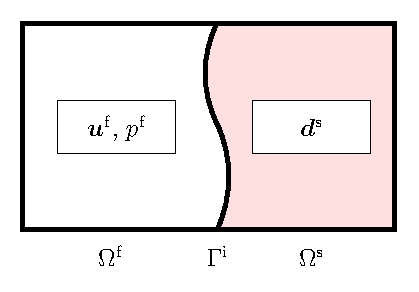
\includegraphics{fig/coupled_system_f_s}
\caption{Coupled FSI problem with fluid and structure domain and a common interface. In the boxes the main variables of each field are given.}
\end{center}
\end{figure}


\subsection{Time integration}

Only implicit time integration implemented for structure and fluid

\begin{itemize}
\item Structure -- Gen. Alpha.

\item Fluid -- one-step-\(\theta\), BDF2
\end{itemize}

They algorithms in \verb|fsi_fluid(), fsi_structure()| are copies of existing single field time integrators.

\section{ALE and Fixed-Grid Methods}

Currently, only Arbitrary Lagrangian Eulerian (ALE) methods are implemented, tested and in use. Fixed grid methods are in preparation and will be added, once they are ready for general usage.


\section{Partitioned algorithms}

One has the choice between several iterative methods and sequential schemes, which however are not generaly applicable for incompressible flow problems.

\paragraph{Fix-Point Iteration}
Fixpunkt
\begin{verbatim}
fsidyn->ifsi==fsi_iter_stagg_fixed_rel_param || (Verschiebungsrelaxation)
fsidyn->ifsi==fsi_iter_stagg_AITKEN_rel_param ||
fsidyn->ifsi==fsi_iter_stagg_steep_desc ||
fsidyn->ifsi==fsi_iter_stagg_AITKEN_rel_force || (Kraftiteration Uli)
fsidyn->ifsi==fsi_iter_stagg_steep_desc_force ||
\end{verbatim}

\paragraph{Newton Iterations}
(Diplomarbeit Markus Schmidtberger)
\begin{verbatim}
fsidyn->ifsi==fsi_iter_stagg_Newton_FD || (Finite Differenzen)
fsidyn->ifsi==fsi_iter_stagg_Newton_I )   (Fixpunkt ohne Relax)
\end{verbatim}

\paragraph{unused}
\begin{verbatim}
fsidyn->ifsi==fsi_iter_stagg_CHEB_rel_param ||
\end{verbatim}

\paragraph{Sequential Algorithms}
Sequential algorithms do not requeire an iteration which make them cheap. However they have a severe time step restriction and might not be applicable for interation involving incompressible flow.
\begin{verbatim}
basic sequentiel staggered scheme
sequential staggered scheme with predictor
\end{verbatim}


\section{Coupling for Matching and Non-Matching Grids}

\subsection{Matching Grids}
Matching grids means that fluid and structure nodes are located at the very same position along the interface und can directly exchange values like velocities or forces.

Calculation of surface forces in 2d and 3d is done either using the integration
\begin{equation}
\int_\Omega \sigma \vec{n} \mathrm{d}\Omega
\end{equation}
or by using consistent nodal forces following Förster


\subsection{Non-Matching Grids}

\subsection{Mortar Methods}
Mortar (Semesterarbeit Firl, Betr. Förster)

the implemented version compiles, but the test fails (Structur: No convergence in maxiter steps)


It should be implemented/reorganized again using the Trilinos library Moertel.

\subsection{Interpolation}
Interpolation (Semesterarbeit Florian Henke (Kuettler))
Einschalten per DEFINES Flag!!
nur für \verb|hex8,hex27,tet4,tet10|





\section{Single field solvers}

In the following all single field solvers that currwtnly work in the FSI setting are briefly reviewed.

\subsection{Fluid}

The working horse so far has been the stabilized equal order Q1Q1 and Q2Q2 finite element fluid solver.

There are also fast Elemente of type \verb|FLUID3D_FAST Elemente|

New approaches to be included into the FSI algorithms are inf-sup stable elements and elements using projection methods (Küttler)

\subsection{Structure}


Wall und Brick Elemente, Shell8


\subsection{ALE mesh dynamics}

The mesh dynamics algorithms are necessary to compute the fluid mesh movement in the interior of the fluid domain.

It's possible to run the pure ALE mesh to test `mesh materials' (\verb|ale_dyn_control.c|)

\subsubsection{Materials \& Element types}
\paragraph{2D}

Springs, Laplace, Linear FE, Linear FE mit versteifendem J, 2step
Elementtypen
QUAD4, QUAD8, QUAD9, TRI3, TRI6

\paragraph{3D}

Lin. Elastisch
Elementtypen
HEX8, HEX20, TET4, TET10


\section{Tests}
\subsubsection{FSI Tests}
\begin{verbatim}
ffsi_ow3D.dat
ffsi_ow3D_usfem_ca.dat
ffsi_ow3D_usfem_ca_sub2.dat
ffsi_ow3D_usfem_ca_sub2_sd2.dat
ffsi_ow3D_usfem.dat
ffsi_ow3D_usfem_sub2.dat
fsi_mtr_dc4x4.dat                           --> Mortar Kopplung -->
fsi_ow32x32.dat
fsi_ow32x32_force.dat
fsi_ow32x32_sd.dat
fsi_ow32x32_usfem_2xaztec.dat
fsi_ow32x32_usfem.dat
fsi_ow3D_usfem.dat
fsi_tank20x10.dat
fsi_tank3D.dat
fsi_tank3D_par.dat
\end{verbatim}

\subsubsection{ALE tests}

\begin{verbatim}
ale2_nln.dat
ale2_nln_sub4.dat
ale_3d_hourg.dat
ale_3d_hourg_sub2.dat
ale_3d_oll.dat
ale_3d_sd2.dat
ale_3d_sd.dat
ale_3d_umfpack.dat
ale_3d_umfpack_fastass.dat
\end{verbatim}

